\subsection*{Coordenadas Polares}

%---------------  coordenadas polares -------------------------

\begin{frame}[label=fun-vet]{Coordenadas Polares}

Um sistema de \dt{coordenadas polares} é estabelecido da seguinte forma:

\begin{enumerate}
\item Fixamos um ponto no plano, conhecido como \dt{polo} (ou origem), denotado por $O$.

\item Fixamos uma semi-reta a partir de $O$, chamada \dt{eixo polar}.
\end{enumerate}

As \dt{coordenadas polares} de ponto {\color{red}$P$} do plano são formadas por um par ordenado $(r,\theta)$, sendo $r$ a distância de {\color{red}$P$} a $O$ e $\theta$ o ângulo entre o eixo polar e a reta $OP$.
\medskip

\centering
\begin{tikzpicture}
\tikzset{>=latex}

\coordinate (A) at ({2*cos(45)},{2*sin(45)});
\coordinate (O) at (0,0);
\coordinate (i) at (2,0);

\pic[draw,angle eccentricity=1.5,->] {angle = i--O--A};

\draw[->] (0,0) -- (3,0) node[right] {eixo polar};

\node[thick] at (0.8,0.3) {$\theta$};
\draw[very thick,blue] (0,0) -- ({2*cos(45)},{2*sin(45)});

\node at (0.5,1) {$r$};
\node[right] at (A) {$(r,\theta)$};
\fill[red] (A) circle (2pt);

\node[left] at (0,0) {$O$};
  
\end{tikzpicture}


		\end{frame}
%%%%%%%%%%%%%%%%%%%%%%%%%%%%%%%%%%%%%%%%%%%%%%%%%%%%%%%		

\begin{frame}[label=polar]

\begin{block}{Convenções}
\begin{itemize}
\item Um ângulo é \dt{positivo} se for medido no sentido anti-horário a partir do eixo polar e {\color{red}negativo} se for medido no sentido horário.

\item $(0,\theta)$ representa o {\color{blue}polo} para qualquer valor de $\theta$.

\item Se $r<0$, a coordenada $(r,\theta)$ corresponde ao simétrico, em relação à origem, do ponto $(|r|,\theta)$.


\centering

\begin{tikzpicture}
\tikzset{>=latex}

\coordinate (A) at ({2*cos(45)},{2*sin(45)});
\coordinate (O) at (0,0);
\coordinate (i) at (2,0);
\coordinate (B) at ({2*cos(45+180)},{2*sin(45+180)});

\pic[draw,->,angle radius=1cm] {angle = i--O--A};

\pic[draw,->] {angle = i--O--B};

\draw[->] (0,0) -- (3,0) node[right] {eixo polar};

\node[thick] at (1.2,0.3) {$\theta$};
\draw[very thick,dashed] (0,0) -- ({2*cos(45)},{2*sin(45)});

\node at (0.5,1) {$|r|$};
\node[right] at (A) {$(|r|,\theta)$};
\fill[black] (A) circle (2pt);

\node[below] at (0,0) {$O$};

\draw[very thick,blue] (0,0) -- ({2*cos(45+180)},{2*sin(45+180)});

\node[left] at (B) {$(r,\theta)$};
\fill[red] (B) circle (2pt);
\node at ({0.8*cos(90+45)},{0.8*sin(90+45)}) {$\theta +\pi$};
  
\end{tikzpicture}
\end{itemize}
\end{block}

\end{frame}

\begin{frame}[label=polar]
\begin{exe}
Marque os pontos cujas coordenadas polares são dadas
\begin{multicols}{4}
\begin{enumerate}[a]
	\item $(1,5\pi/4)$
	
	\item $(2,3\pi)$
	
	\item  $(2,-2\pi/3)$
	
	\item $(-3,3\pi/4)$  \medskip
\end{enumerate}
\end{multicols}
\end{exe}

\only<1>{
\begin{center}
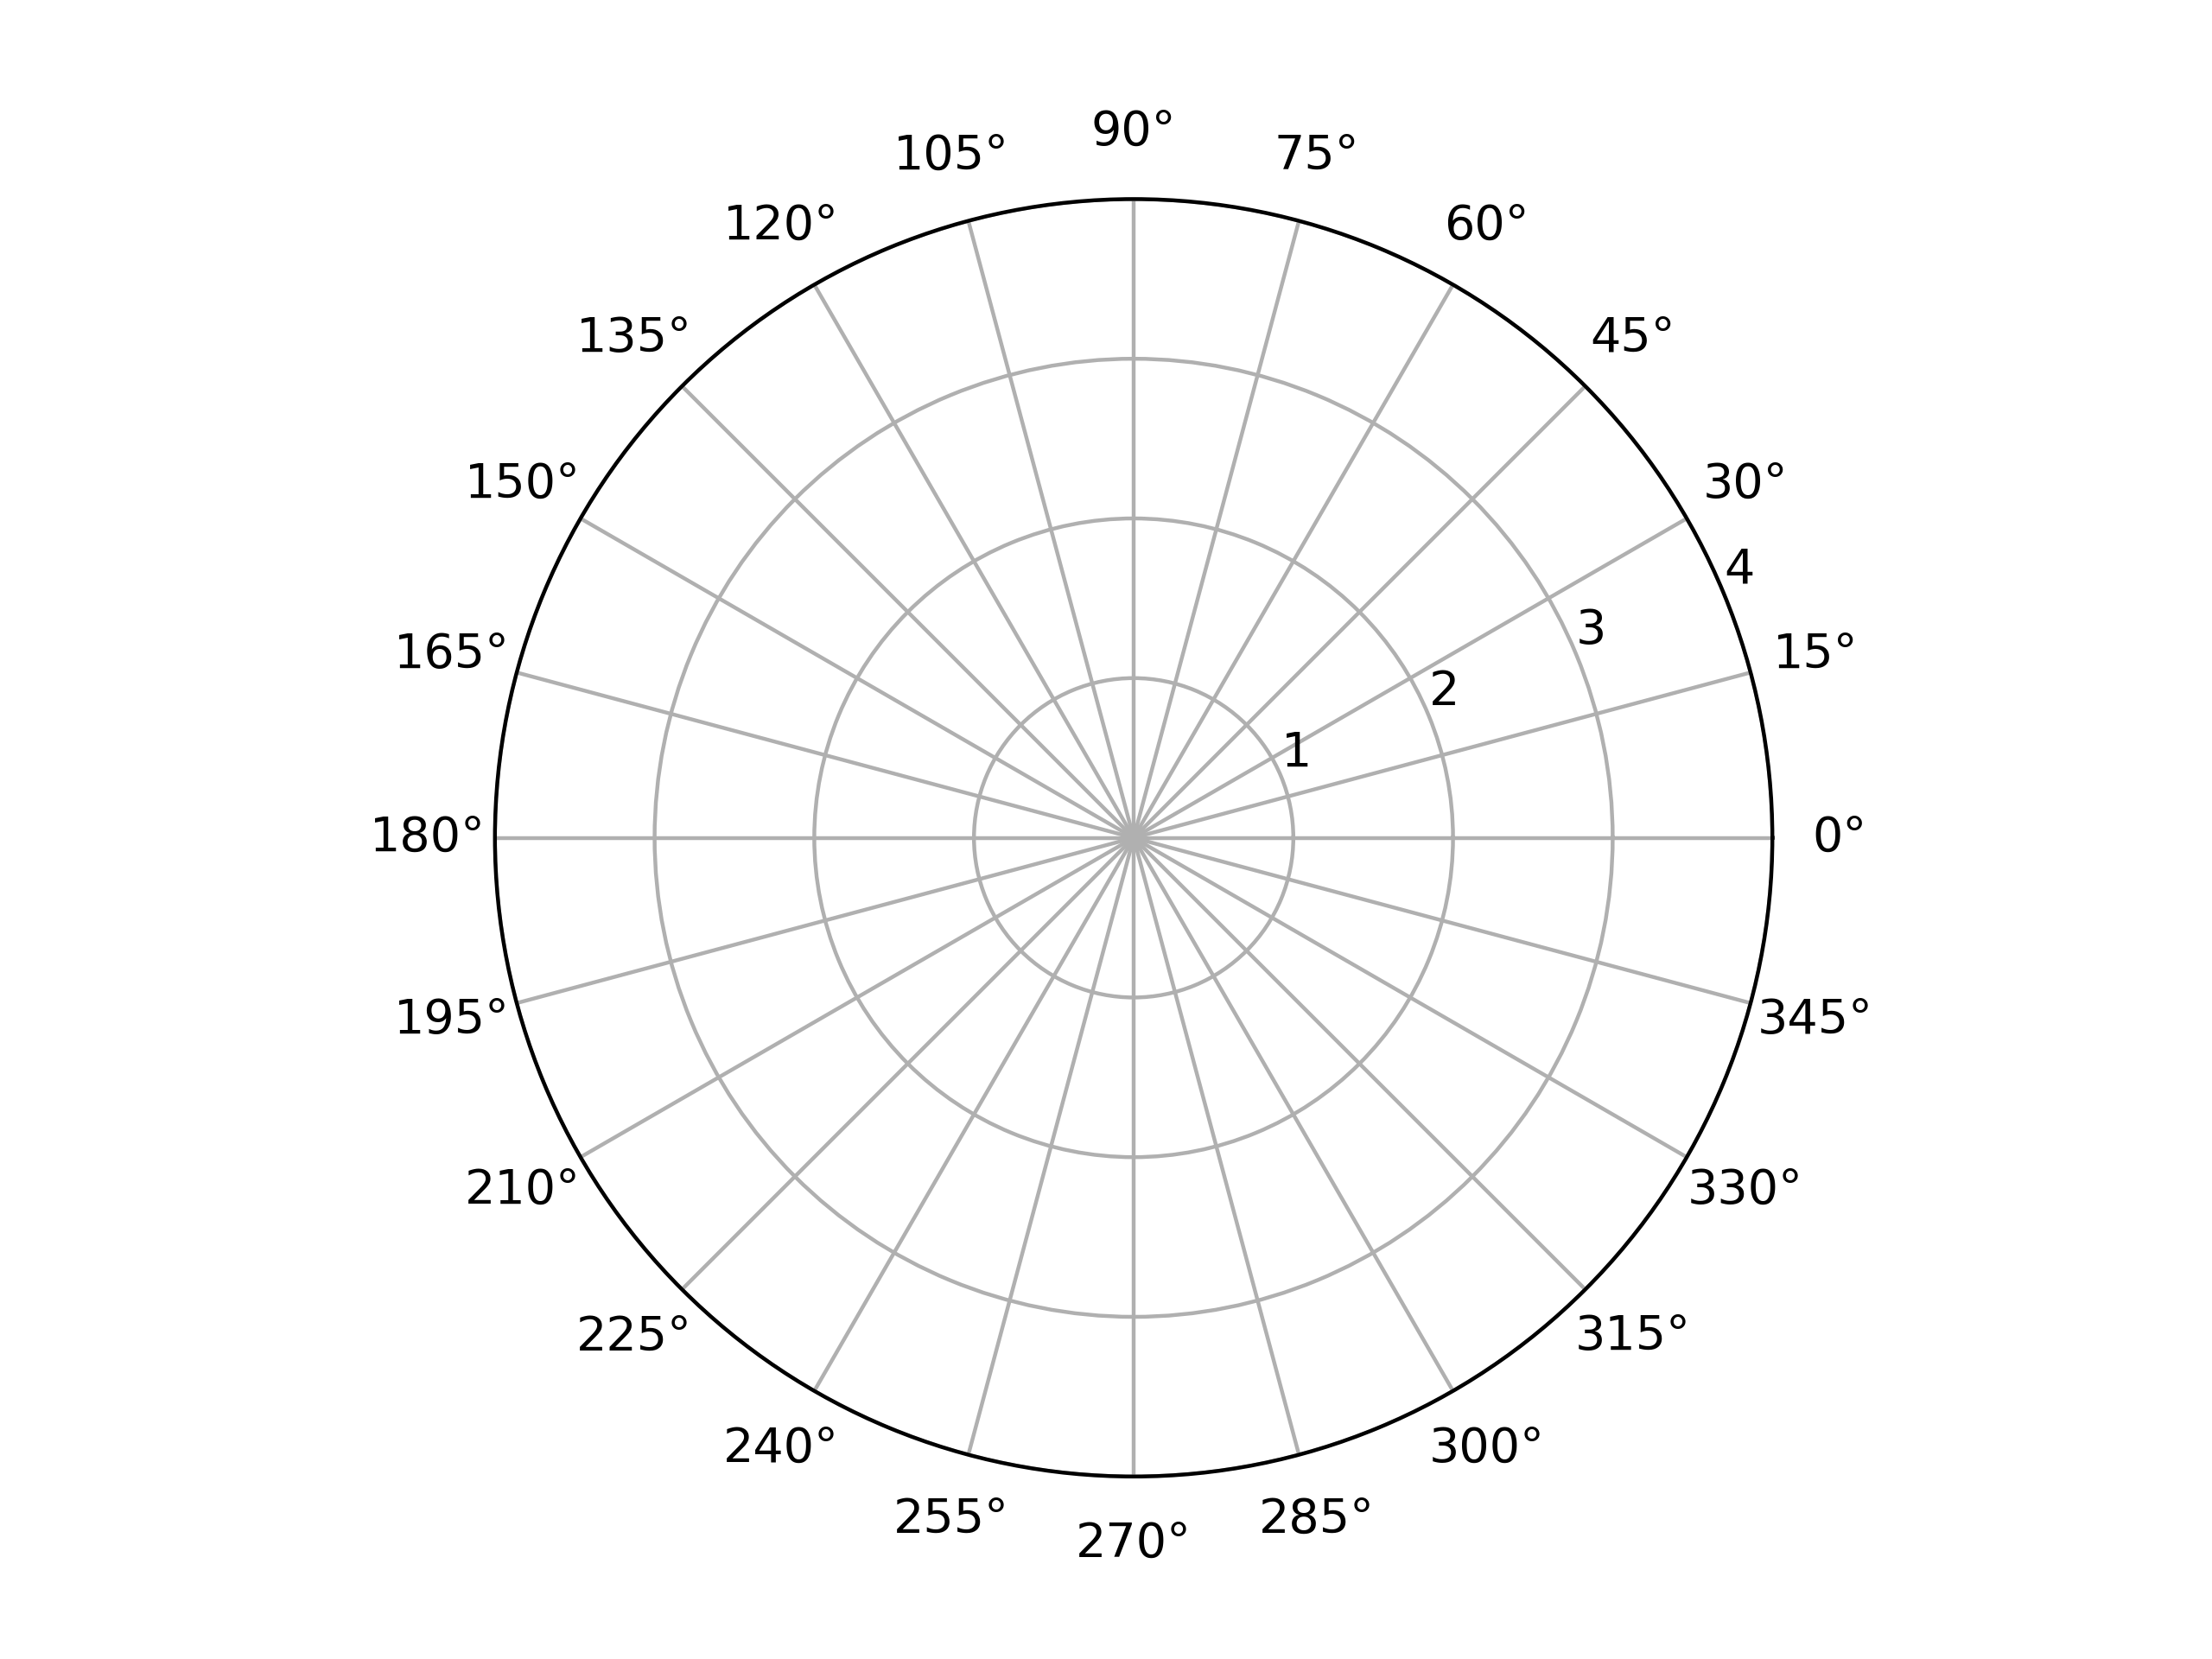
\includegraphics[scale=.5]{figuras/polar/polar-grid.png}
\end{center}
}

\only<2>{
\begin{center}
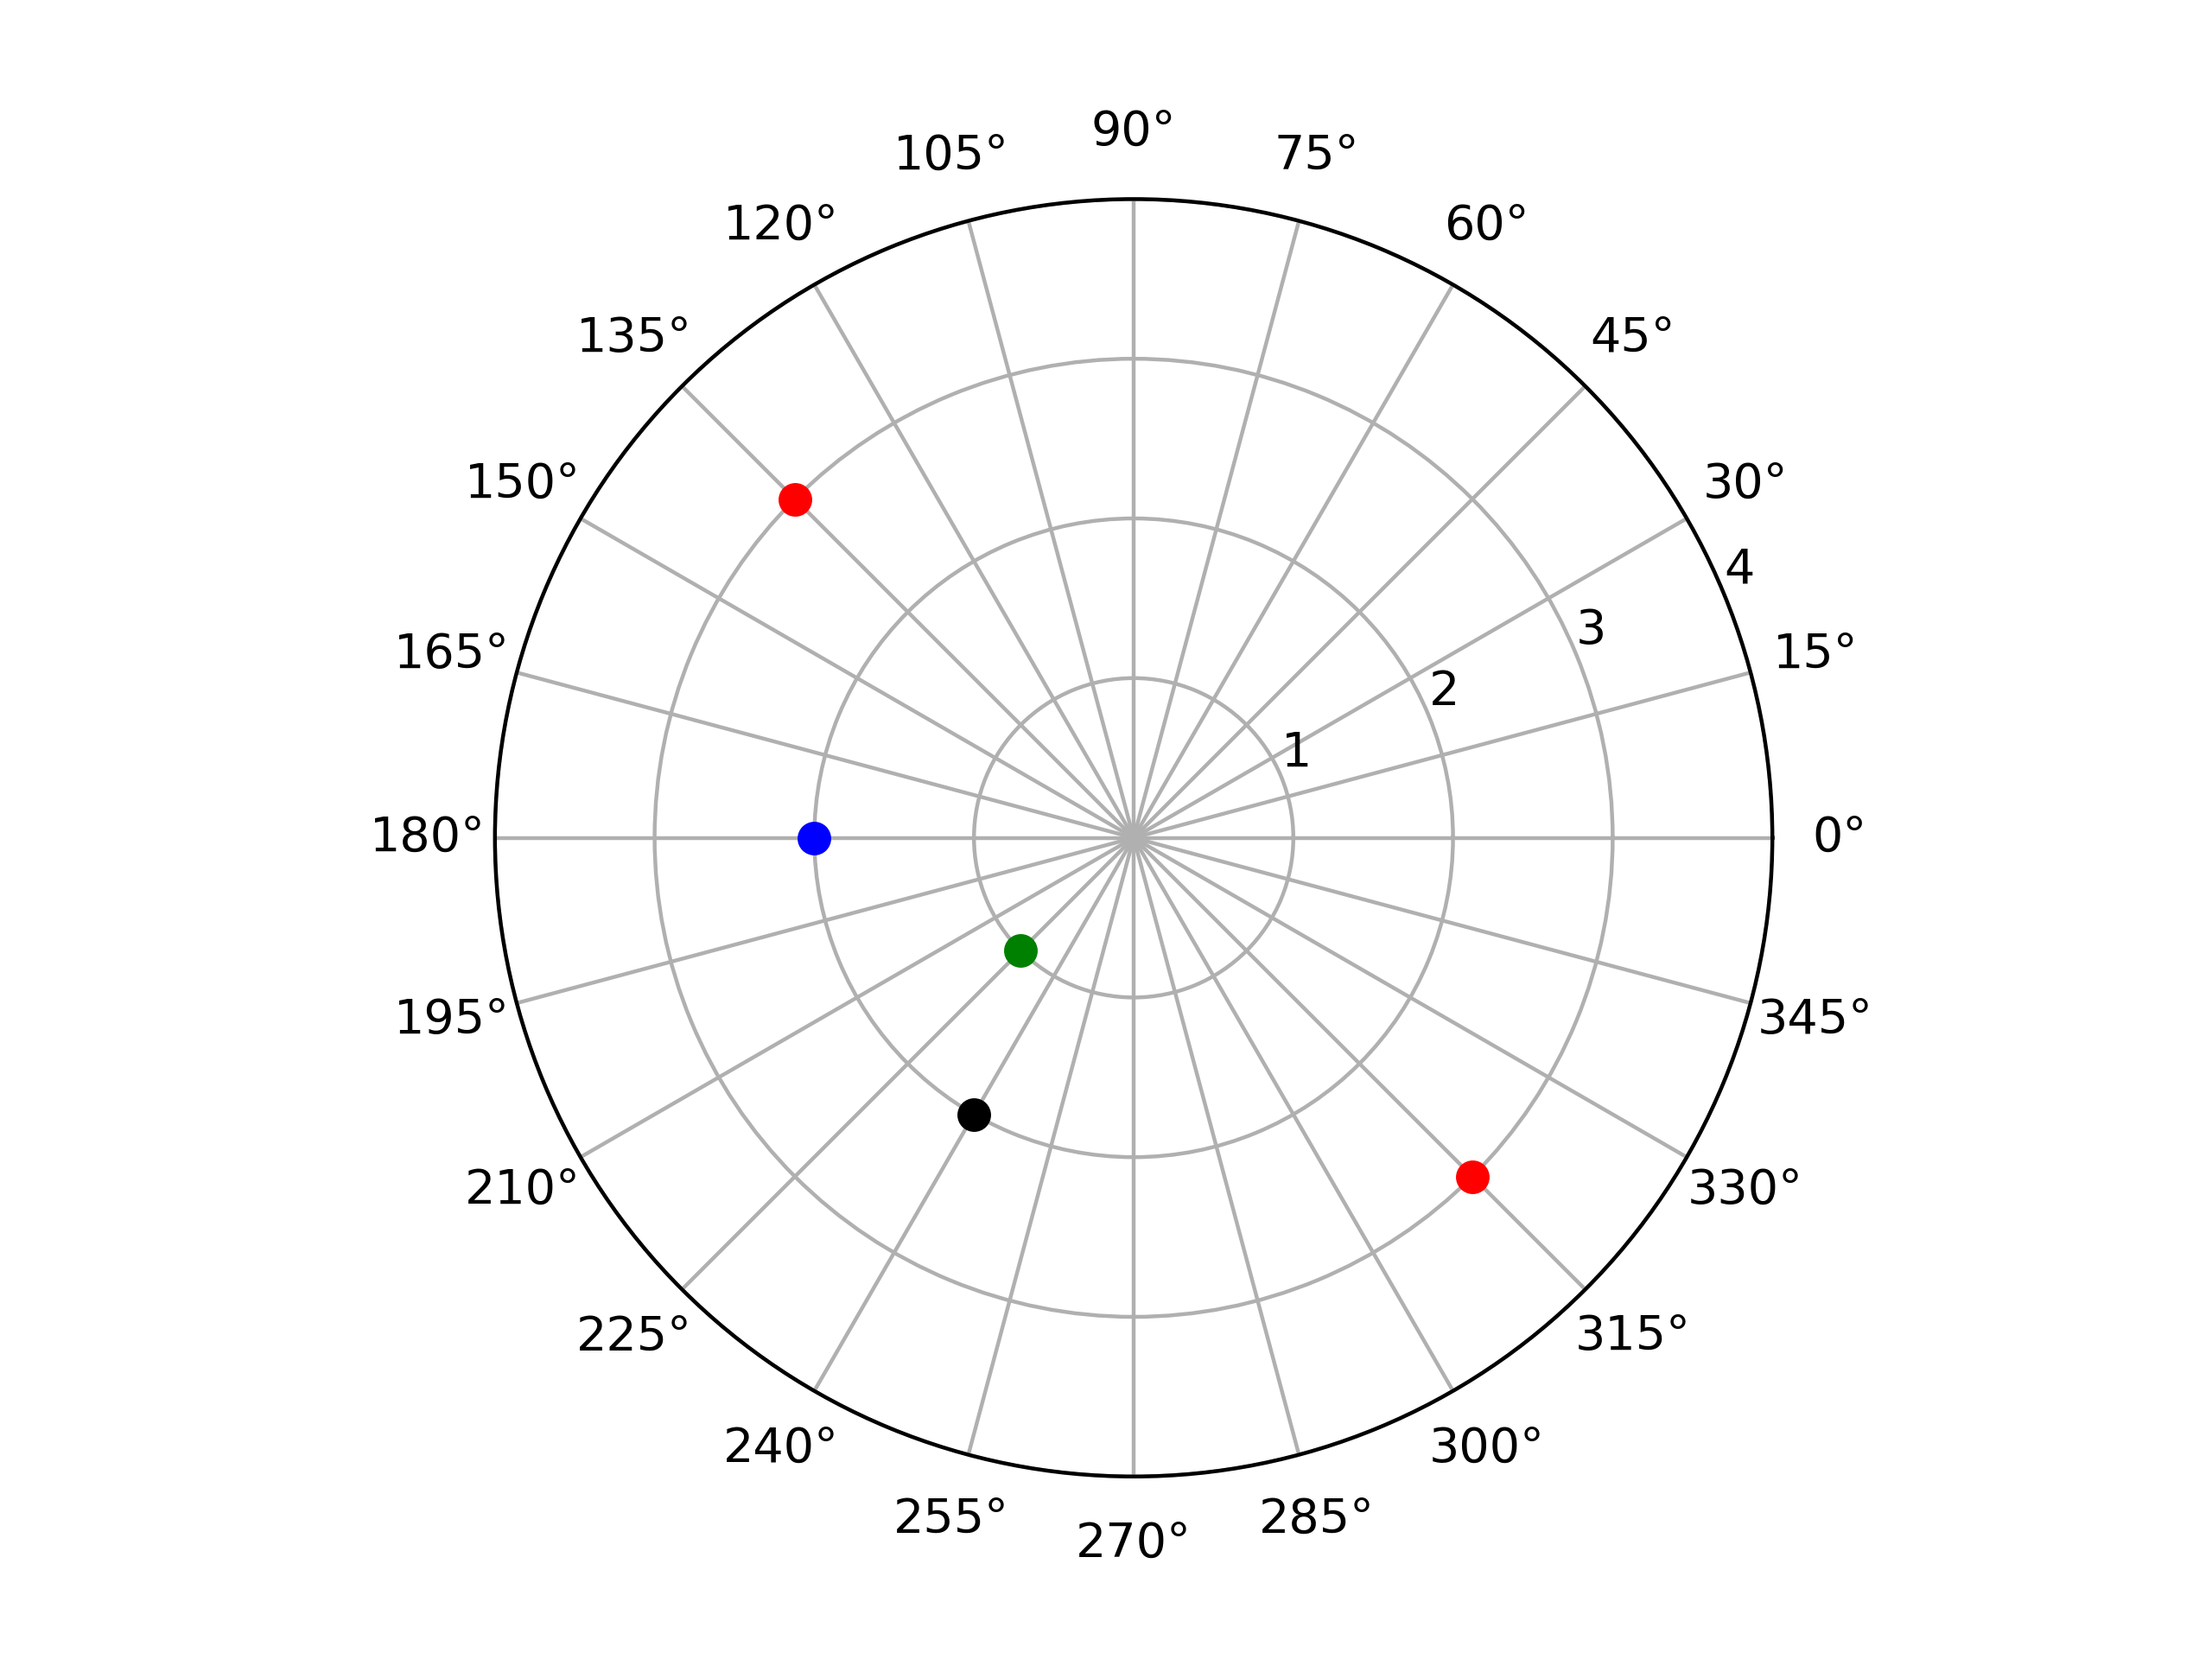
\includegraphics[scale=.5]{figuras/polar/polar-grid2.png}
\end{center}
}


\end{frame}

\begin{frame}[label=fun-vet,fragile=singleslide]
\begin{block}{ }
\begin{small}
\begin{pyverbatim}
import numpy as np
import matplotlib.pyplot as plt

ax = plt.axes(projection='polar')
angulos=list(range(0, 360, 15))
raios = [1, 2, 3, 4]

# plota os pontos
plt.polar(5*np.pi/4,1, 'g.')
plt.polar(3*np.pi,2, 'b.')
plt.polar(-2*np.pi/3,2, 'k.')
plt.polar(3*np.pi/4,3, 'r.')
plt.polar(3*np.pi/4+np.pi,3, 'r.')

ax.set_thetagrids(angulos) 
ax.set_rgrids(raios)
plt.show()
\end{pyverbatim}
\end{small}
\end{block}


\end{frame}



\begin{frame}[label=fun-vet]{Curvas Polares}
\begin{block}{Relação entre coordenadas cartesianas e polares}

$$x=r\cos \theta, \ \ \ y=r\sen \theta, \ \ \ r^2=x^2+y^2$$
\end{block}

O \dt{gráfico de uma equação polar} consiste em todos os pontos $P$ que têm pelo menos uma representação $(r,\theta)$ cujas coordenadas satisfaçam a equação. 

\begin{exe} Esboce a curva que é representada pelas equações polares abaixo.
%\begin{multicols}{3}
		\begin{enumerate}[a]
		\item $r=2$
		
		\item $\theta=1$
		
%		\item $r=2\cos\theta$

	%	\item $r=1+\cos\theta$ (cardioide)
%		\item $r=\cos 2\theta$ (rosácea de quatro pétalas)
			\end{enumerate}
%\end{multicols}
\end{exe}

\end{frame}

\begin{frame}[label=polar]
\begin{exe} Esboce a curva que é representada pela seguinte equação polar
\[r=1+\cos(\theta) \text{ (cardioide)}\]
\end{exe}


\begin{center}
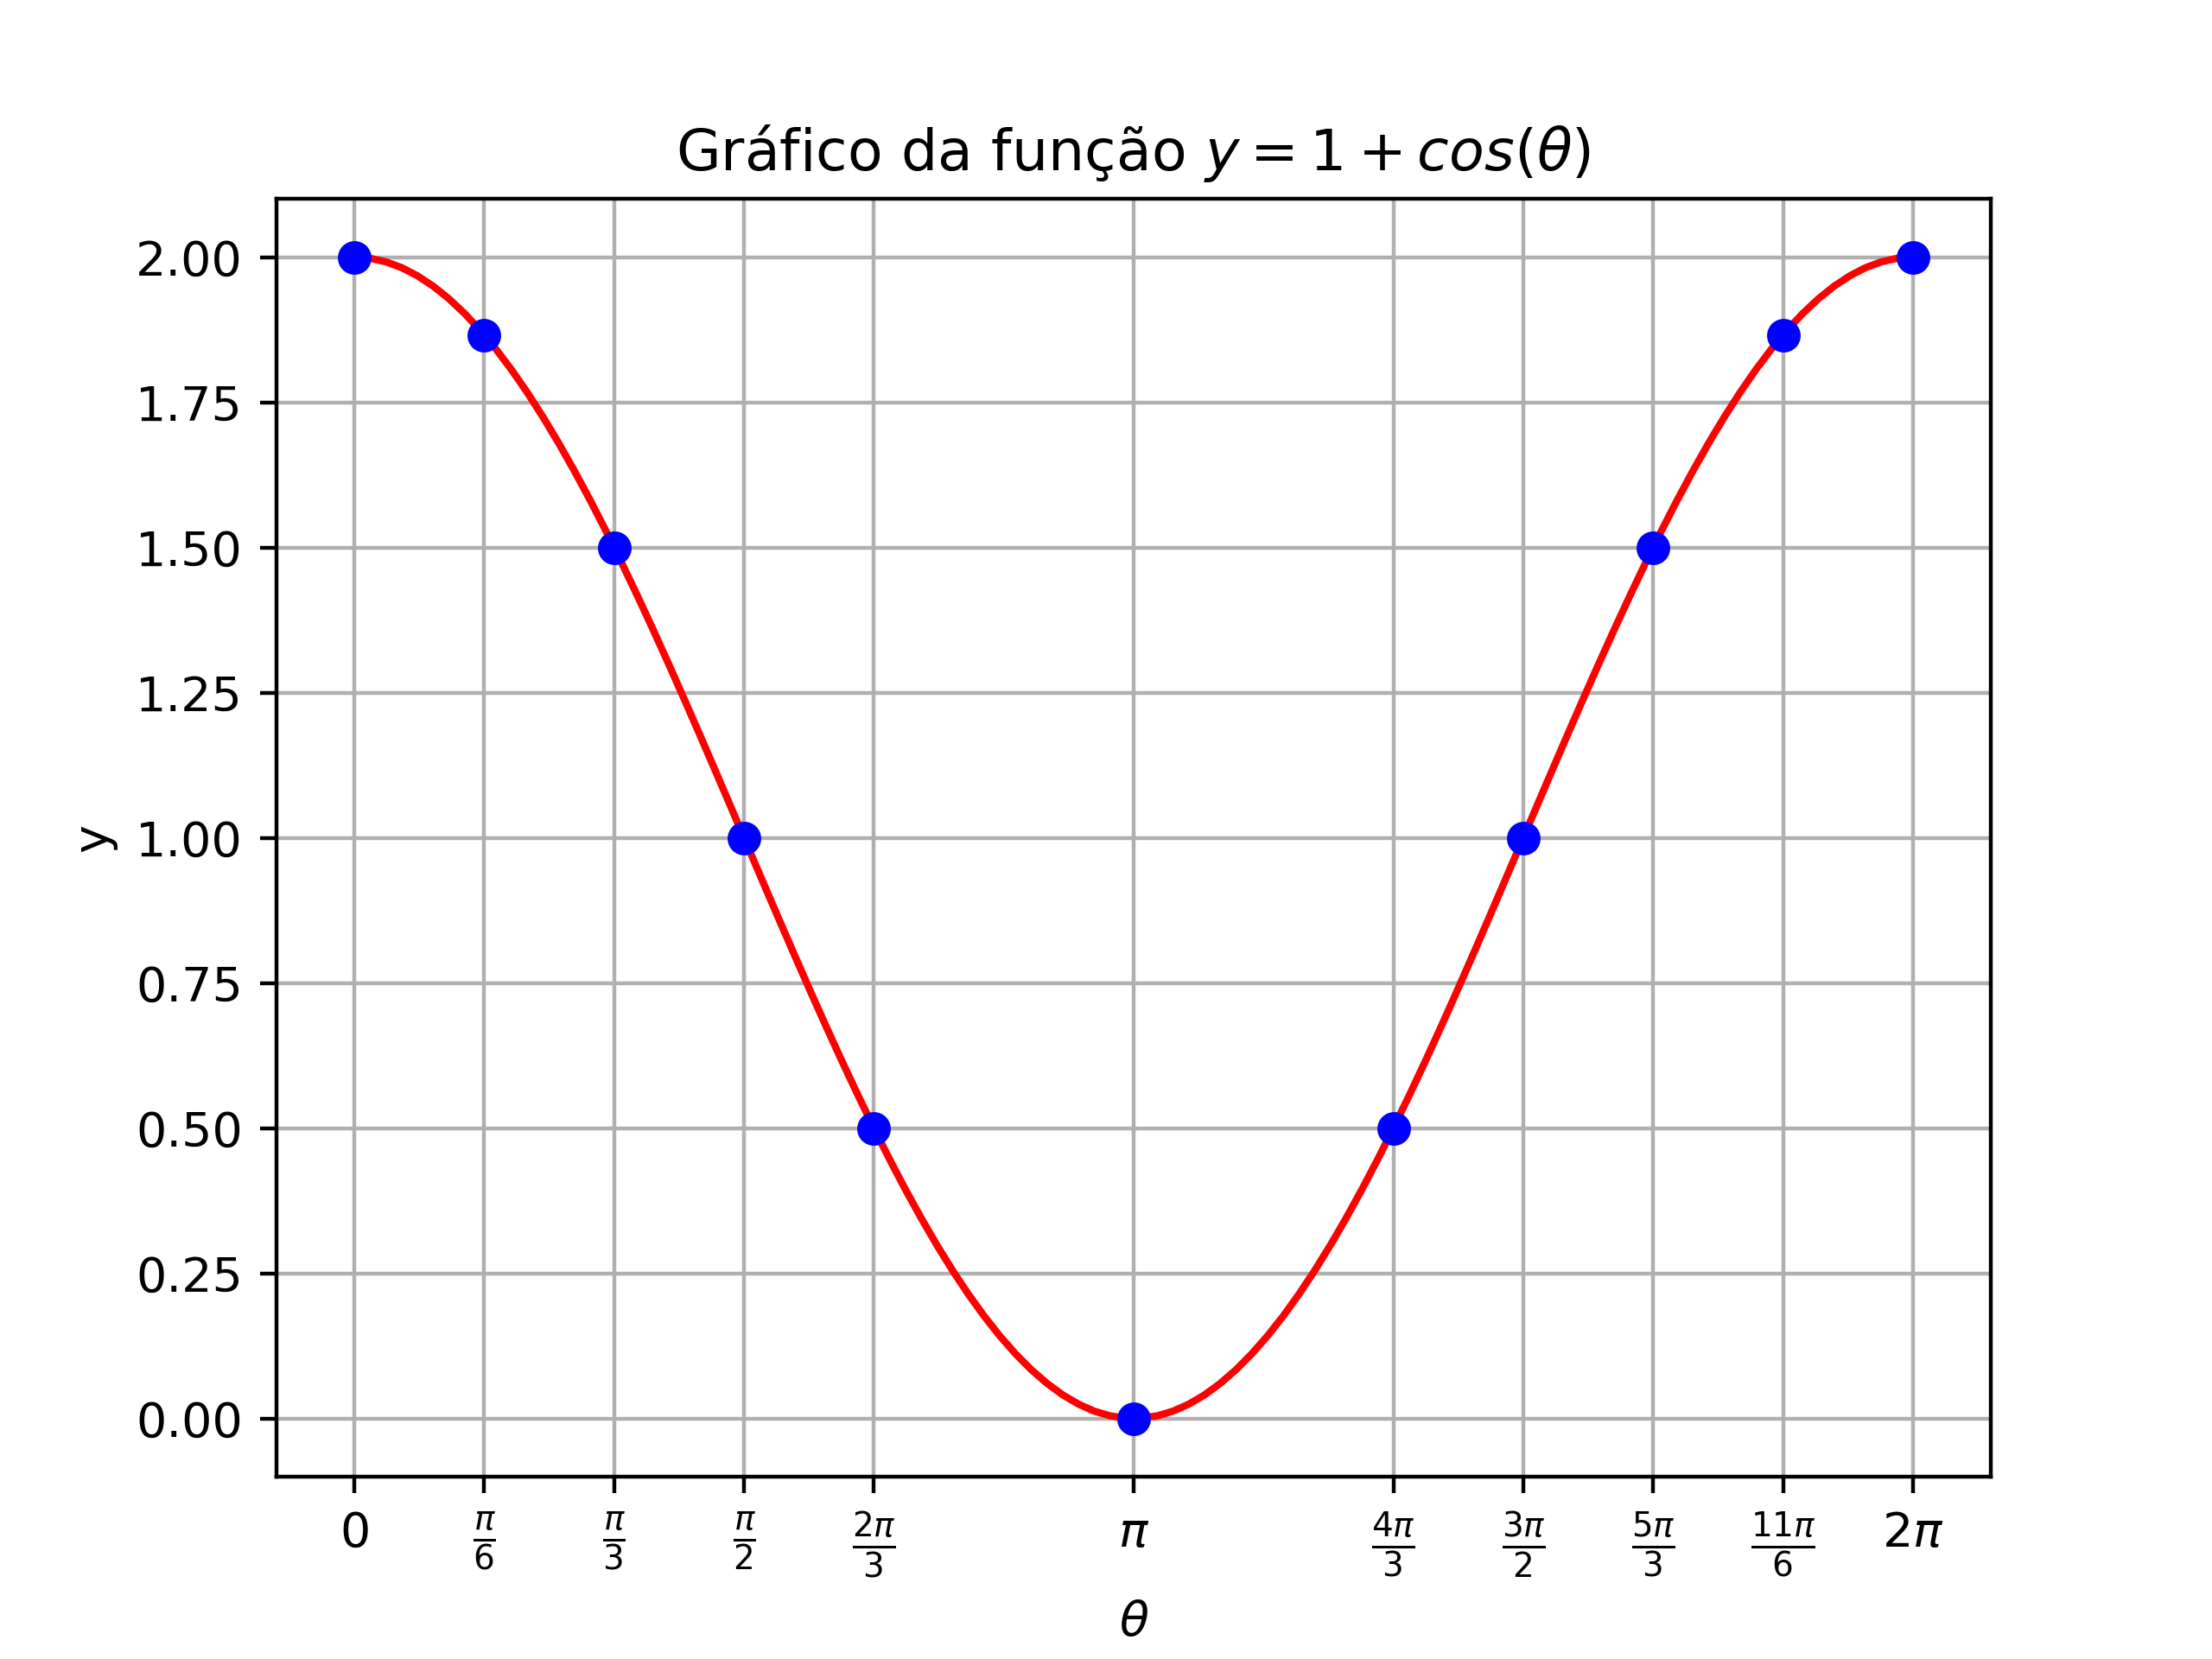
\includegraphics[scale=0.5]{figuras/grafico-aux-cardioide.png}
\end{center}
\end{frame}

\begin{frame}[label=polar]
\only<1>{
\begin{center}
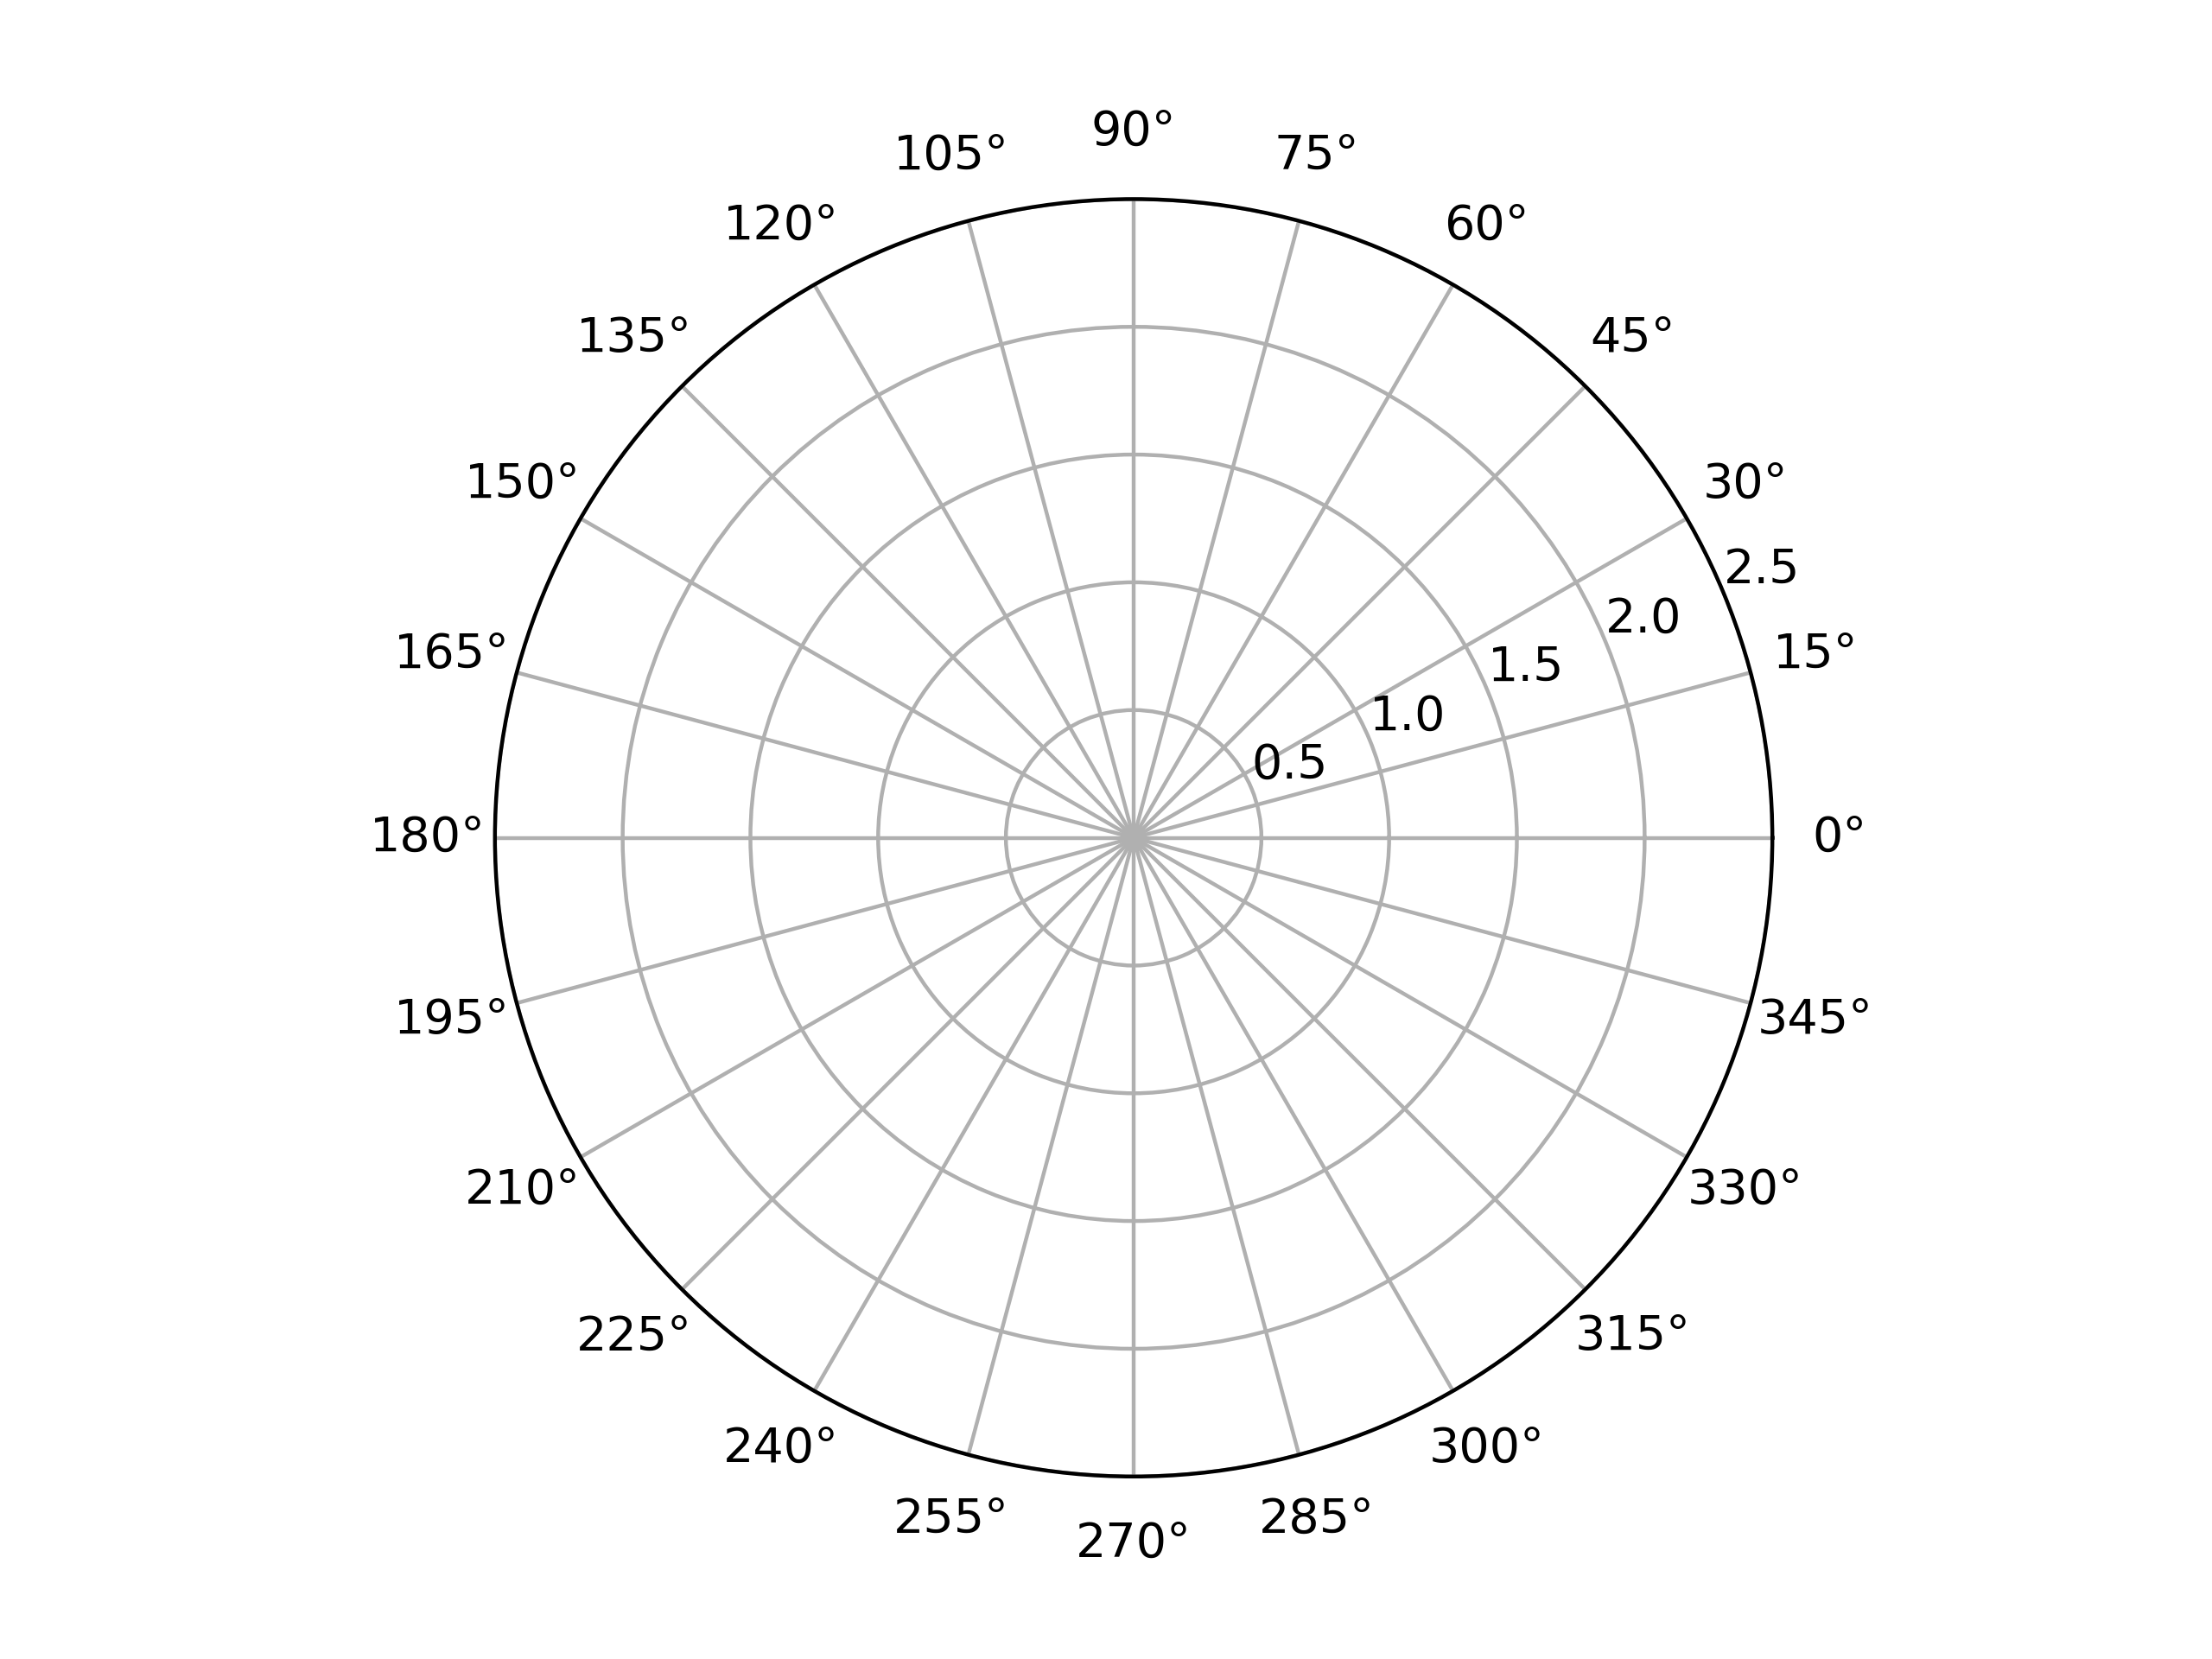
\includegraphics[scale=.7]{figuras/polar/cardioide-grid.png}
\end{center}
}
\only<2>{
\begin{center}
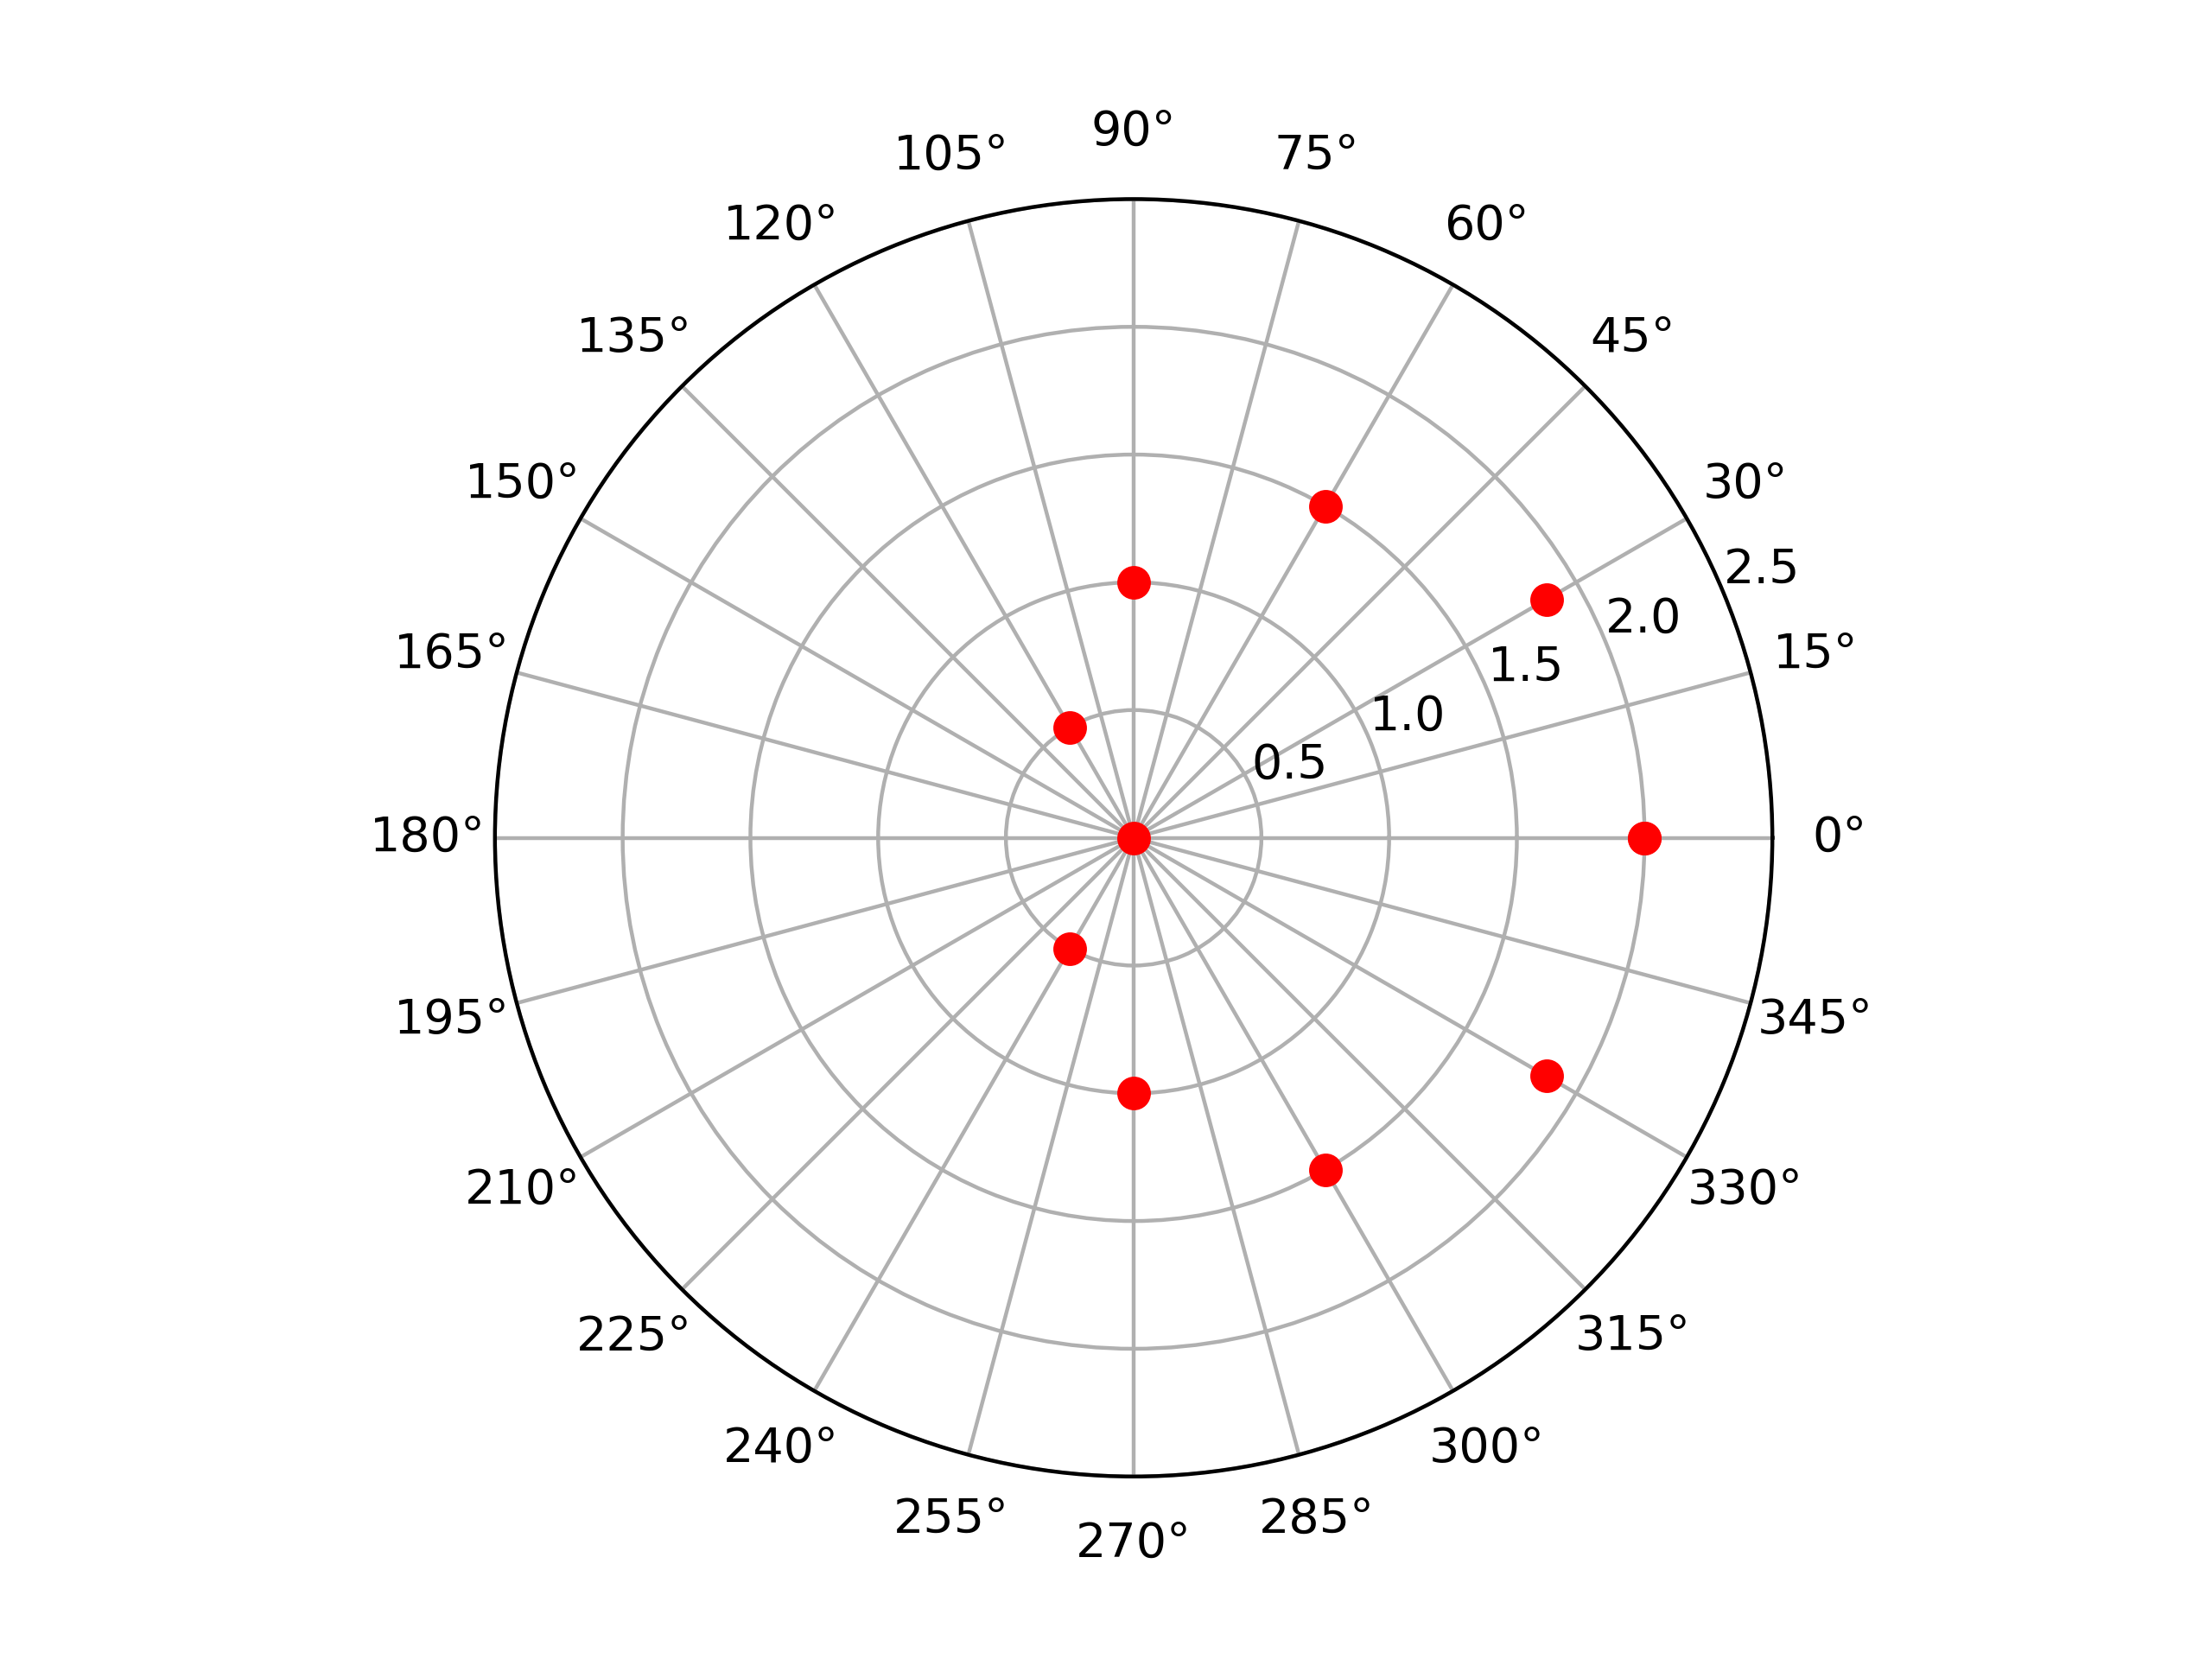
\includegraphics[scale=.7]{figuras/polar/cardioide1.png}
\end{center}
}
\only<3>{
\begin{center}
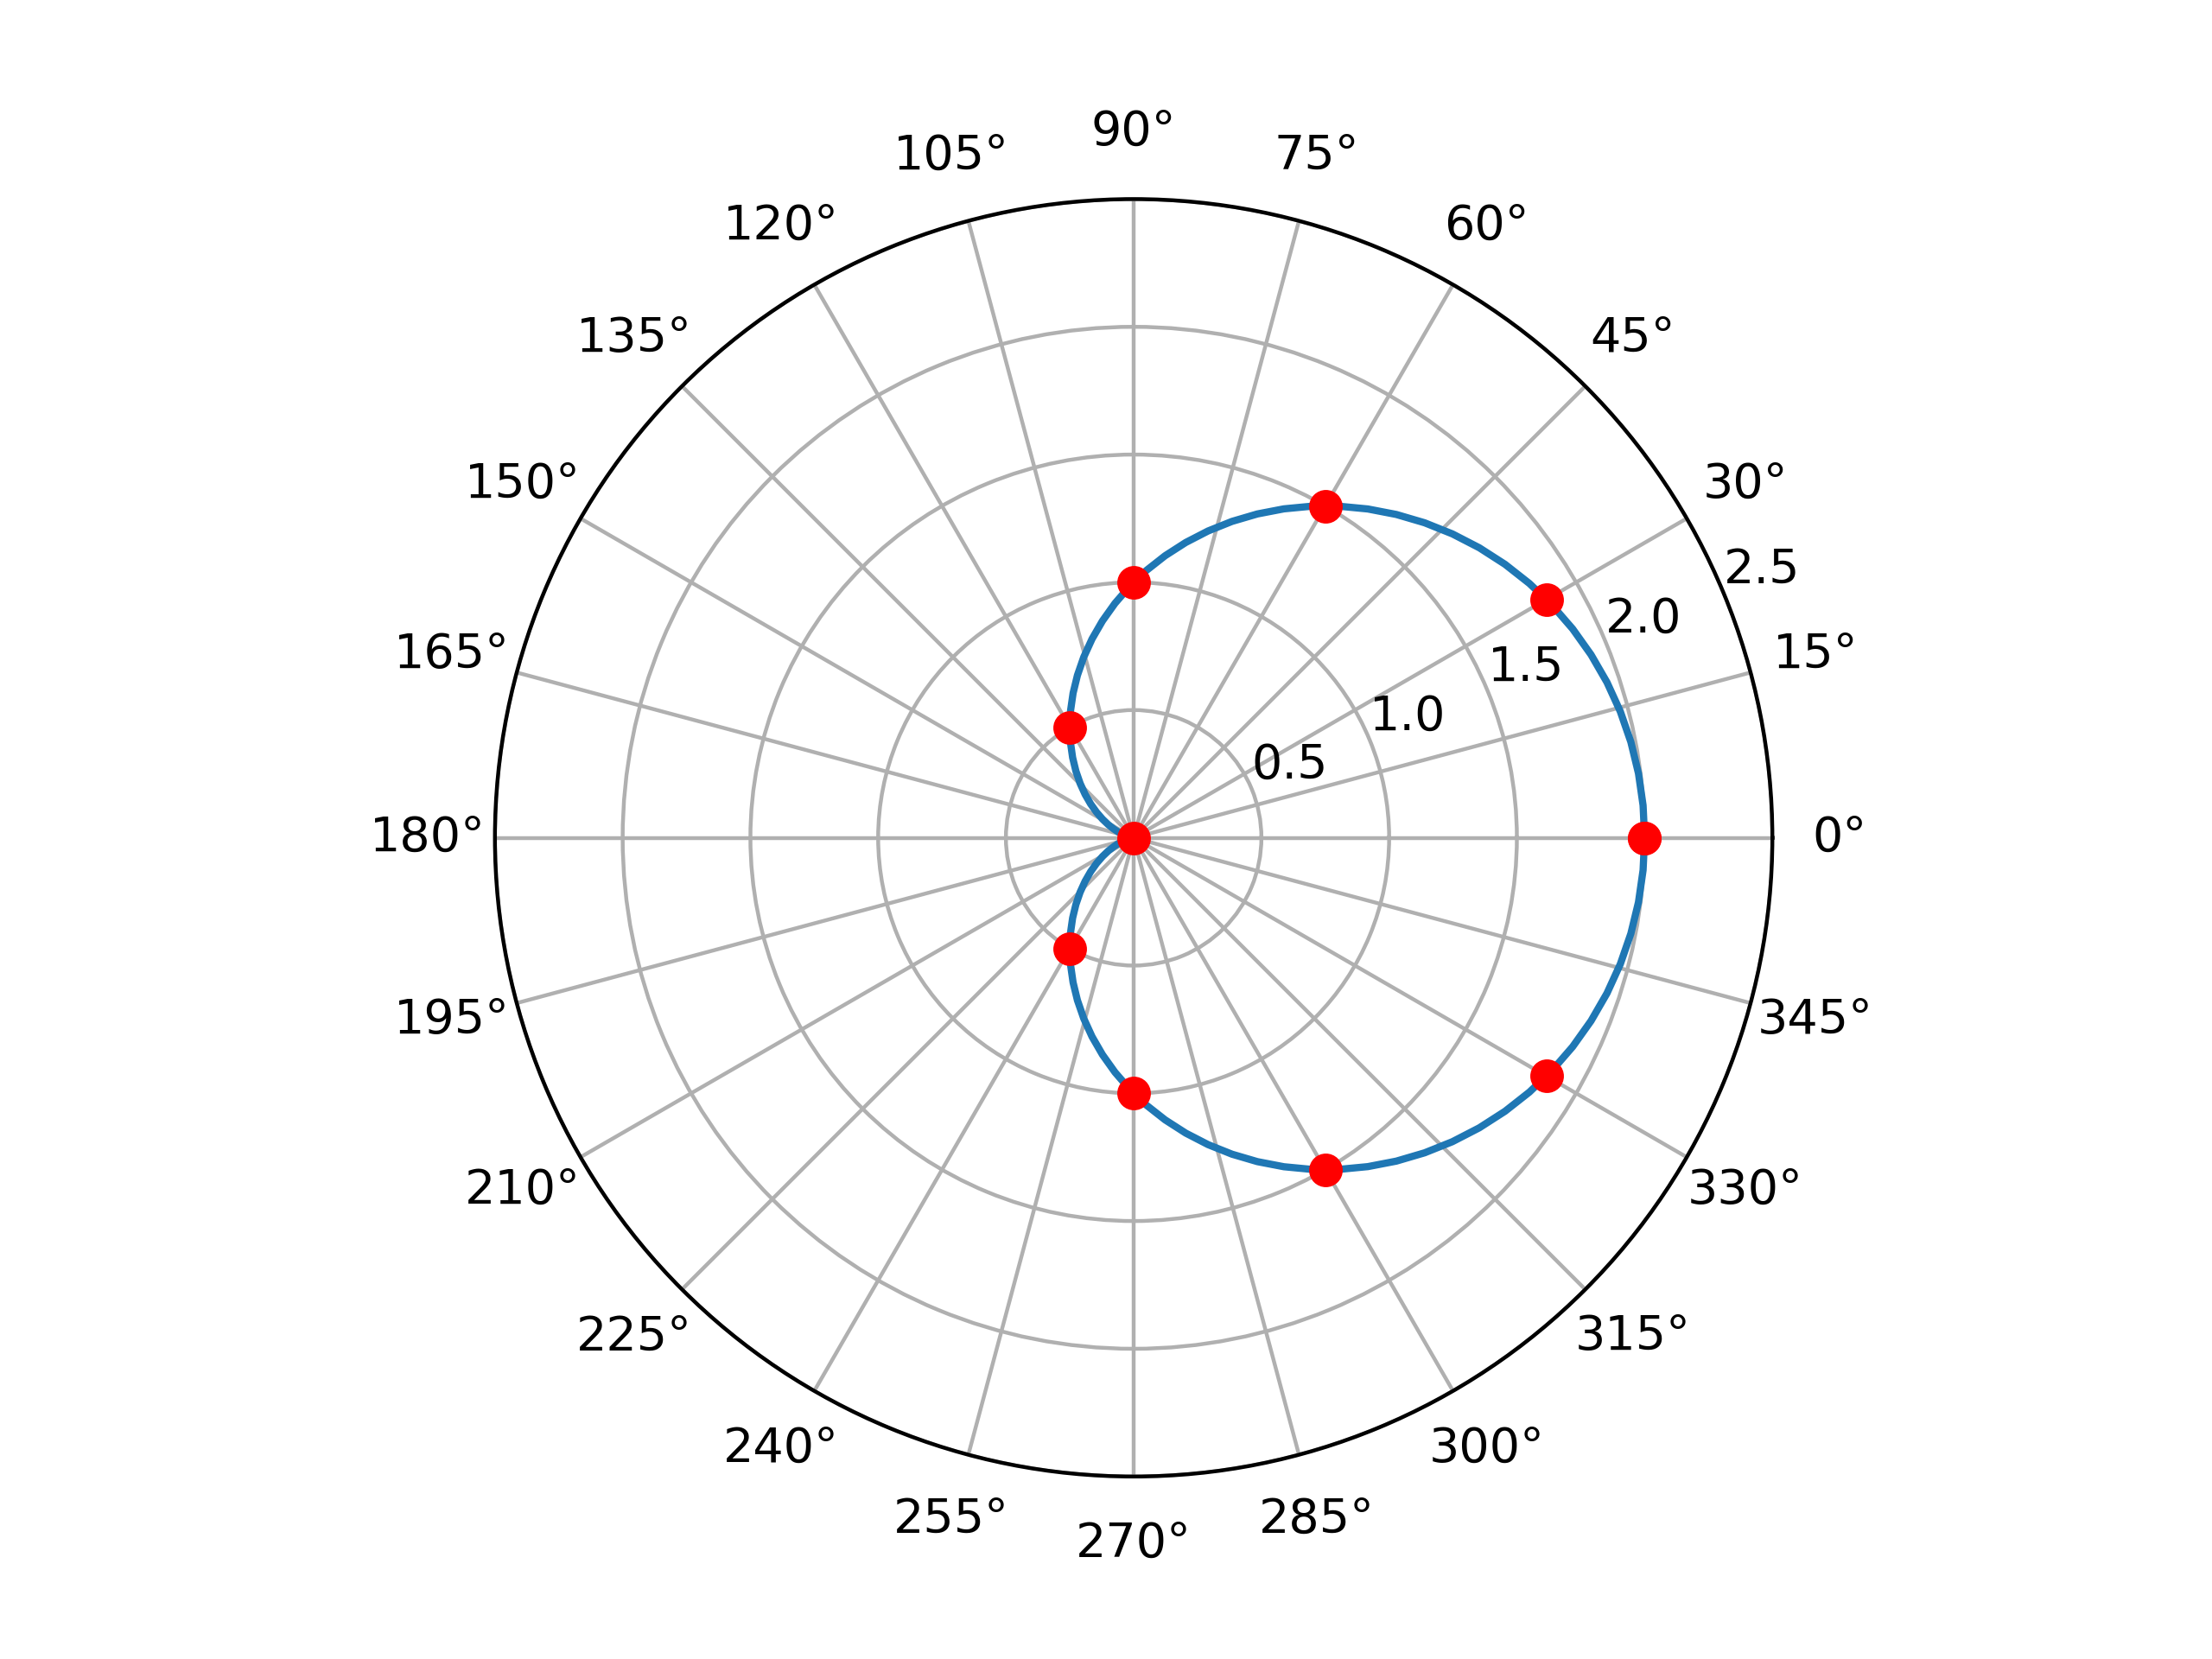
\includegraphics[scale=.7]{figuras/polar/cardioide2.png}
\end{center}
}
\only<4>{
\begin{center}
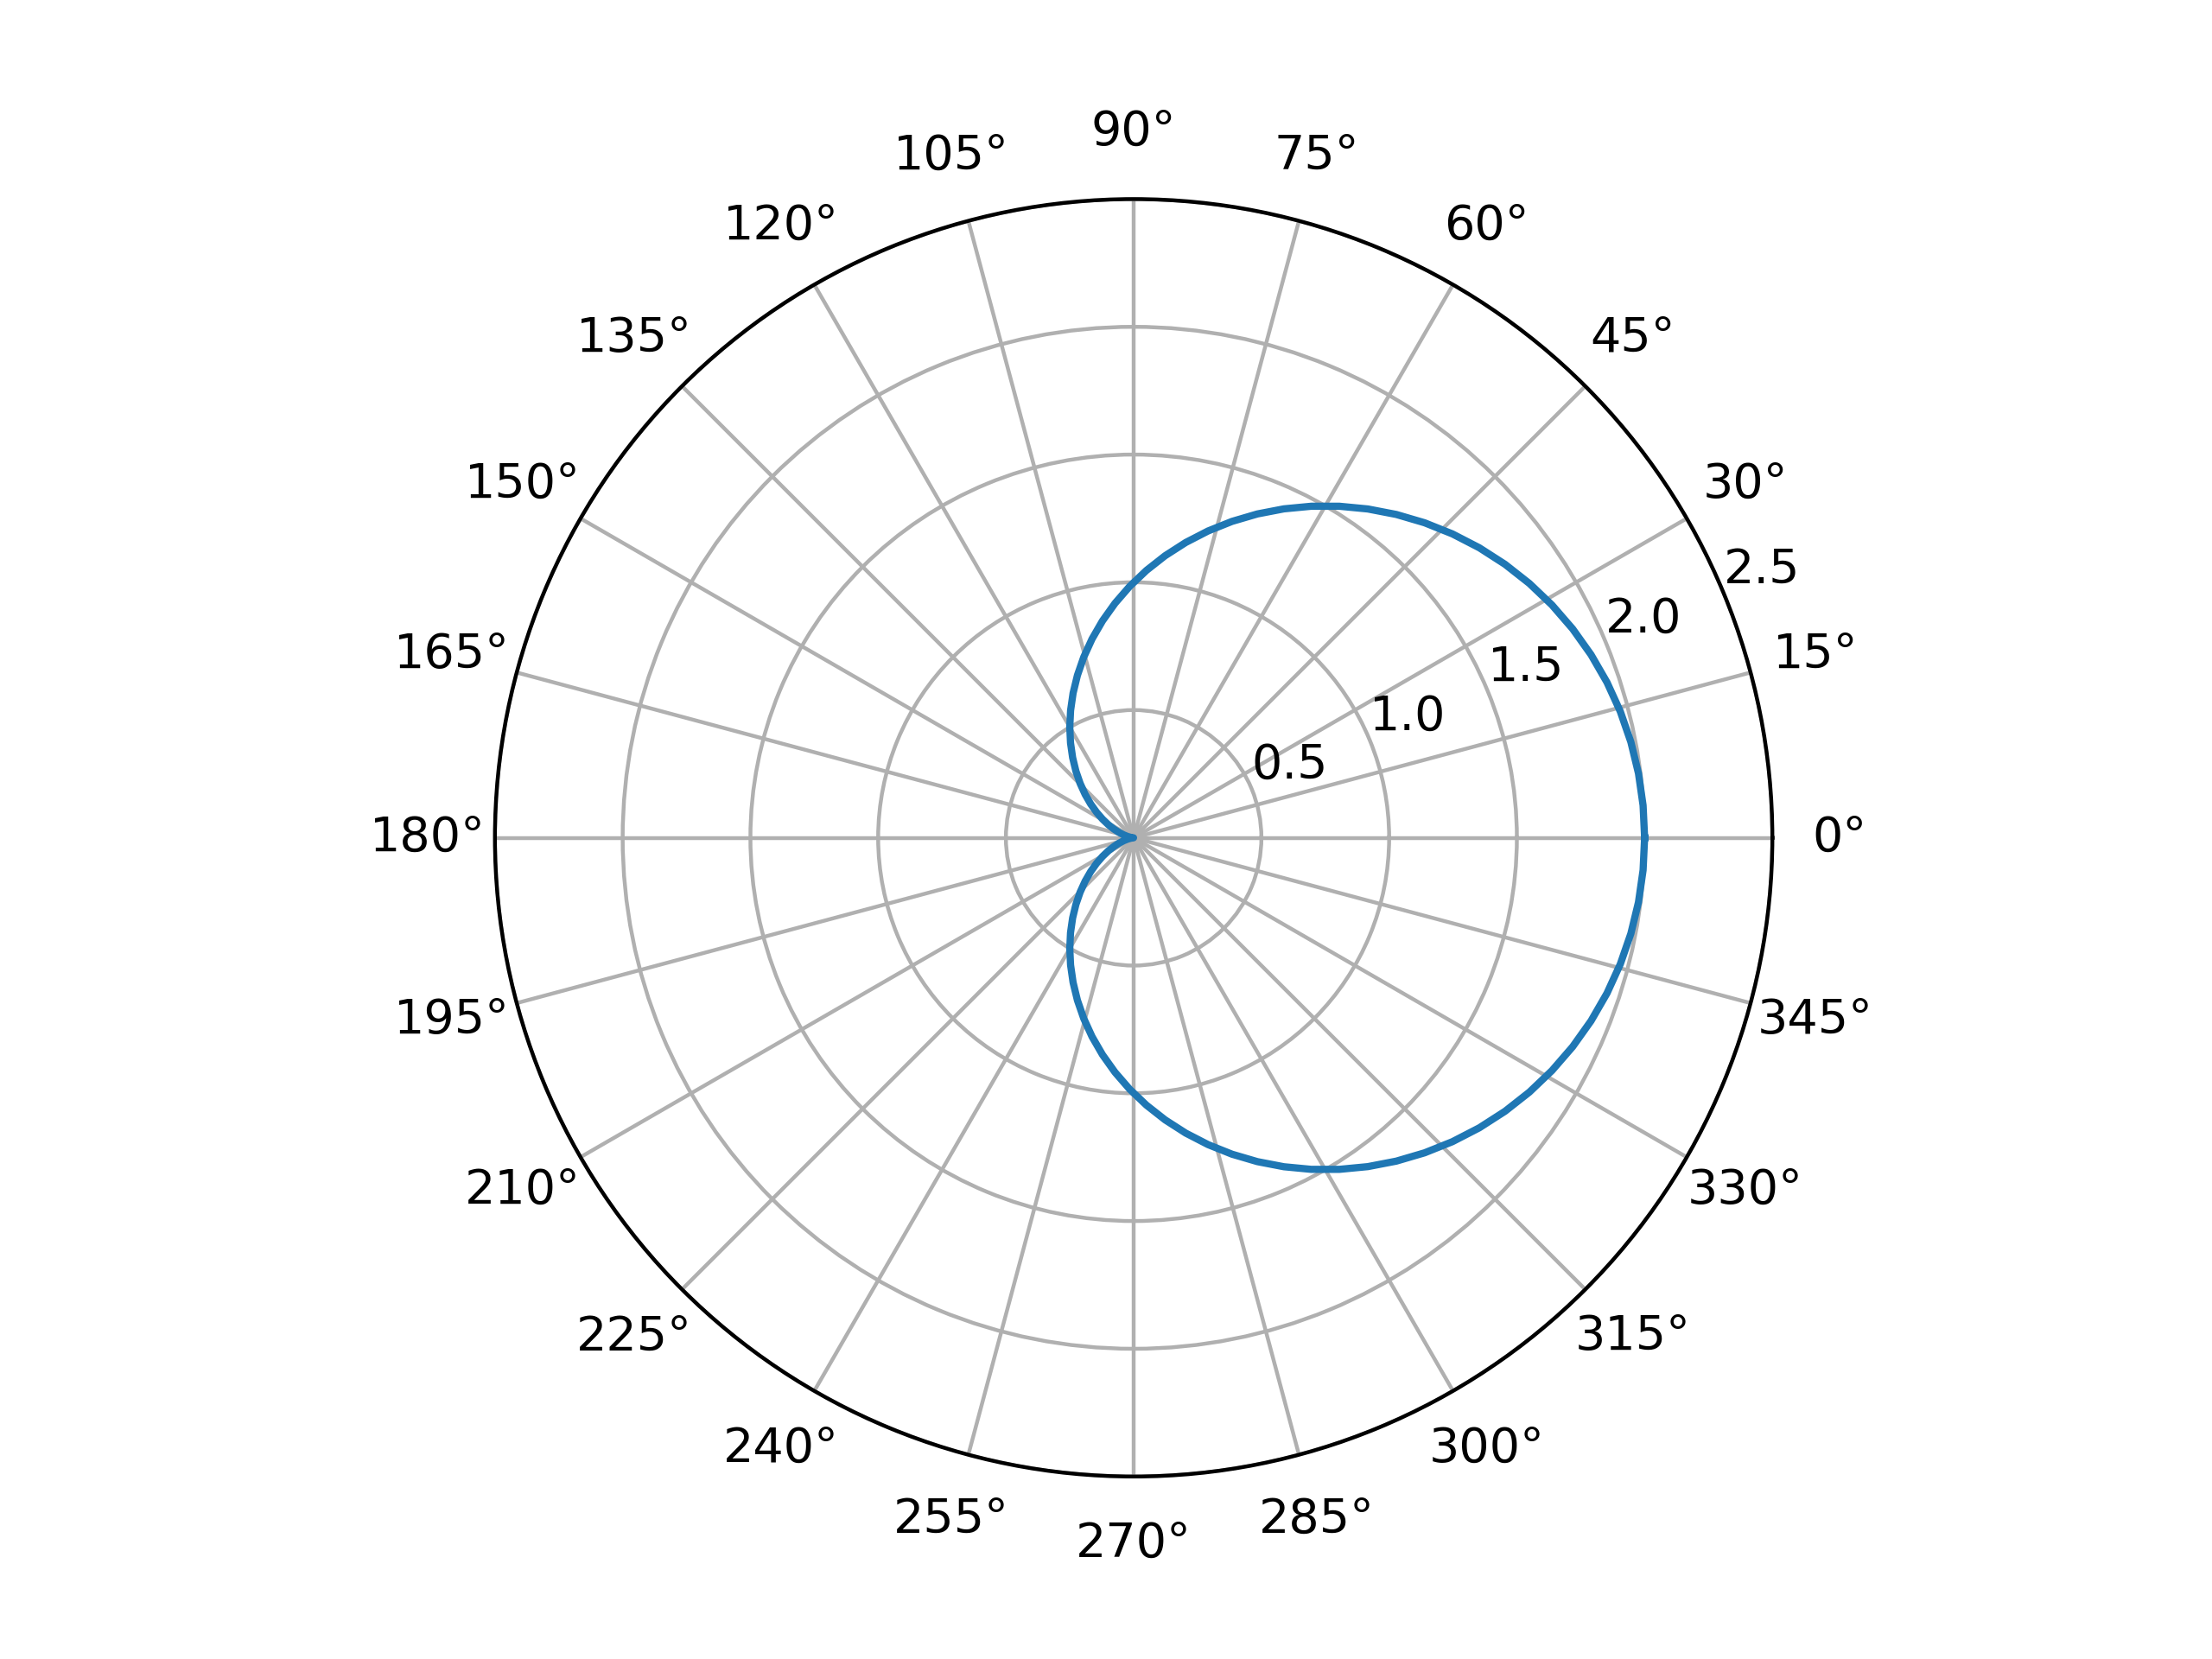
\includegraphics[scale=.7]{figuras/polar/cardioide3.png}
\end{center}
}

\end{frame}

\begin{frame}[label=polar,fragile=singleslide]{Plotando a Cardiode}
\begin{block}{}
\begin{small}
\begin{pyverbatim}
import matplotlib.pyplot as plt
import numpy as np

ax = plt.axes(projection='polar')

#plotar o gráfico
theta= np.linspace(0, 2*np.pi, 100)
r=1+np.cos(theta)
plt.polar(theta, r)

#construir a malha
raios = [0.5,1,1.5,2,2.5]
angulos=list(range(0, 360, 15))
ax.set_thetagrids(angulos) 
ax.set_rgrids(raios)

plt.show()
\end{pyverbatim}
\end{small}
\end{block}


\end{frame}

